\documentclass{standalone}
\usepackage{tikz}
\usetikzlibrary{patterns, positioning}


\begin{document}
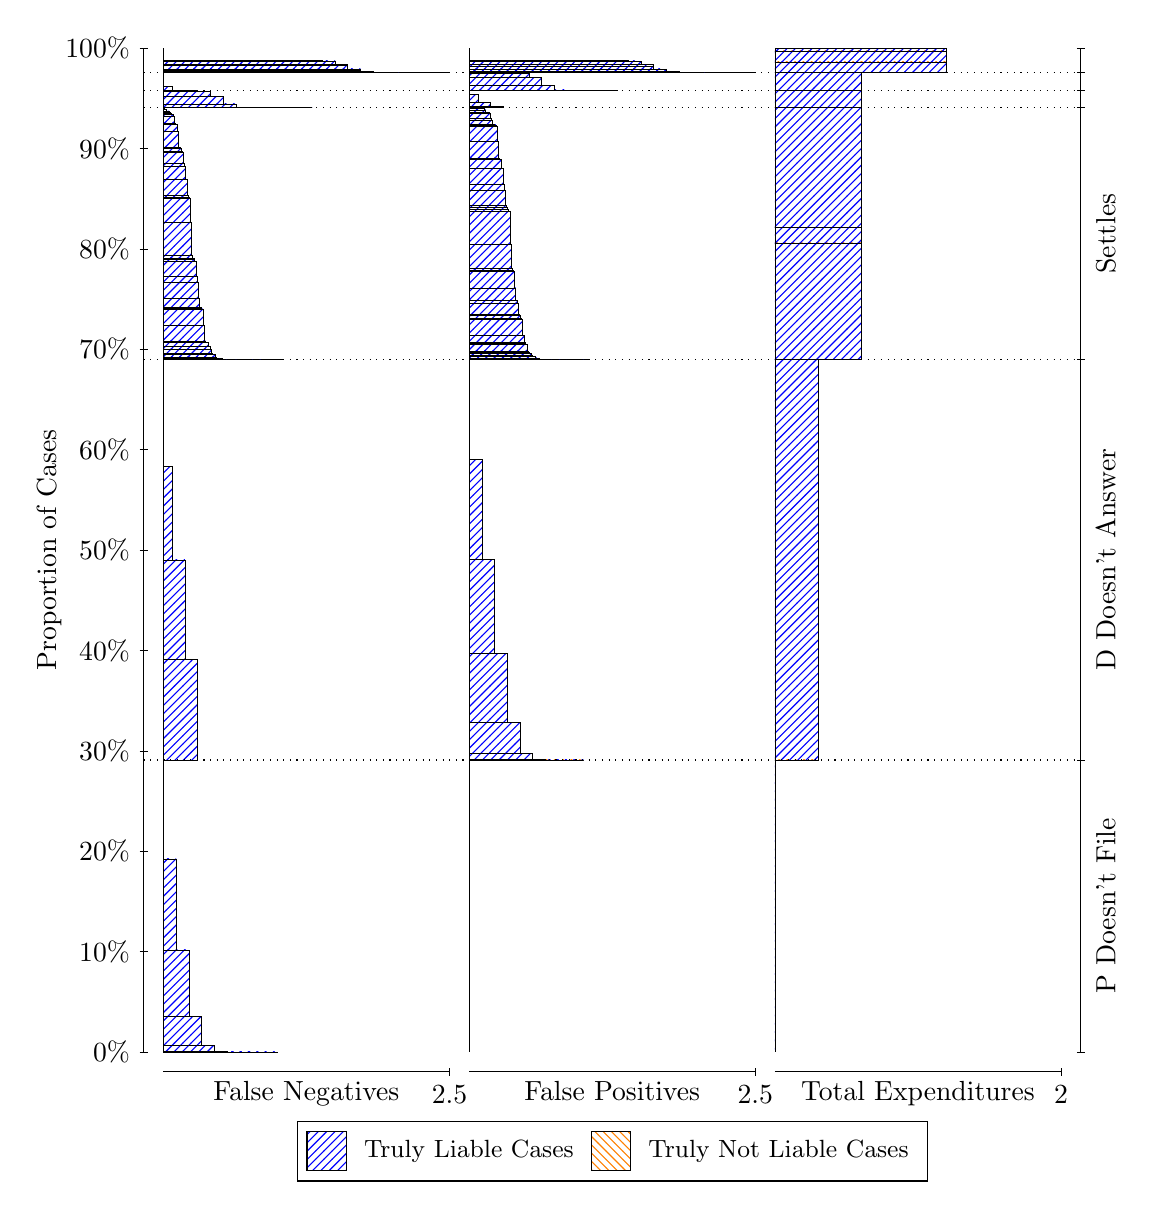
\begin{tikzpicture}
\draw[black, very thin] (1.5,1.75) -- (1.5,14.5);
\node[rotate=90, text=black, anchor=center] at (0.3, 8.125) {Proportion of Cases};
\draw[black, very thin] (1.45,1.75) -- (1.55,1.75);
\node[text=black, anchor=east] at (1.45, 1.75) {0\%};
\draw[black, very thin] (1.45,3.025) -- (1.55,3.025);
\node[text=black, anchor=east] at (1.45, 3.025) {10\%};
\draw[black, very thin] (1.45,4.3) -- (1.55,4.3);
\node[text=black, anchor=east] at (1.45, 4.3) {20\%};
\draw[black, very thin] (1.45,5.575) -- (1.55,5.575);
\node[text=black, anchor=east] at (1.45, 5.575) {30\%};
\draw[black, very thin] (1.45,6.85) -- (1.55,6.85);
\node[text=black, anchor=east] at (1.45, 6.85) {40\%};
\draw[black, very thin] (1.45,8.125) -- (1.55,8.125);
\node[text=black, anchor=east] at (1.45, 8.125) {50\%};
\draw[black, very thin] (1.45,9.4) -- (1.55,9.4);
\node[text=black, anchor=east] at (1.45, 9.4) {60\%};
\draw[black, very thin] (1.45,10.675) -- (1.55,10.675);
\node[text=black, anchor=east] at (1.45, 10.675) {70\%};
\draw[black, very thin] (1.45,11.95) -- (1.55,11.95);
\node[text=black, anchor=east] at (1.45, 11.95) {80\%};
\draw[black, very thin] (1.45,13.225) -- (1.55,13.225);
\node[text=black, anchor=east] at (1.45, 13.225) {90\%};
\draw[black, very thin] (1.45,14.5) -- (1.55,14.5);
\node[text=black, anchor=east] at (1.45, 14.5) {100\%};

\draw[black, very thin] (13.4,1.75) -- (13.4,14.5);
\draw[black, very thin] (13.35,1.75) -- (13.45,1.75);
\node[anchor=west] at (13.35, 1.75) {};
\draw[black, very thin] (13.35,5.4583) -- (13.45,5.4583);
\node[anchor=west] at (13.35, 5.4583) {};
\draw[black, very thin] (13.35,10.547) -- (13.45,10.547);
\node[anchor=west] at (13.35, 10.547) {};
\draw[black, very thin] (13.35,13.745) -- (13.45,13.745);
\node[anchor=west] at (13.35, 13.745) {};
\draw[black, very thin] (13.35,13.959) -- (13.45,13.959);
\node[anchor=west] at (13.35, 13.959) {};
\draw[black, very thin] (13.35,14.187) -- (13.45,14.187);
\node[anchor=west] at (13.35, 14.187) {};
\draw[black, very thin] (13.35,14.5) -- (13.45,14.5);
\node[anchor=west] at (13.35, 14.5) {};

\draw[black, very thin, pattern color=blue, pattern=north east lines] (1.75,1.75) rectangle (3.2033,1.75);
\draw[black, very thin, pattern color=blue, pattern=north east lines] (1.75,1.75) rectangle (3.0419,1.75);
\draw[black, very thin, pattern color=blue, pattern=north east lines] (1.75,1.75) rectangle (2.8804,1.75);
\draw[black, very thin, pattern color=blue, pattern=north east lines] (1.75,1.75) rectangle (2.7189,1.7503);
\draw[black, very thin, pattern color=blue, pattern=north east lines] (1.75,1.7503) rectangle (2.5574,1.7576);
\draw[black, very thin, pattern color=blue, pattern=north east lines] (1.75,1.7576) rectangle (2.3959,1.8367);
\draw[black, very thin, pattern color=blue, pattern=north east lines] (1.75,1.8367) rectangle (2.2344,2.2055);
\draw[black, very thin, pattern color=blue, pattern=north east lines] (1.75,2.2055) rectangle (2.073,3.0459);
\draw[black, very thin, pattern color=blue, pattern=north east lines] (1.75,3.0459) rectangle (1.9115,4.2036);
\draw[black, very thin, pattern color=orange, pattern=north west lines] (1.75,4.2036) rectangle (1.75,4.2036);
\draw[black, very thin, pattern color=blue, pattern=north east lines] (1.75,4.2036) rectangle (1.75,5.4583);
\draw[black, very thin, pattern color=blue, pattern=north east lines] (1.75,5.4583) rectangle (2.186,6.7329);
\draw[black, very thin, pattern color=blue, pattern=north east lines] (1.75,6.7329) rectangle (2.0245,7.9994);
\draw[black, very thin, pattern color=blue, pattern=north east lines] (1.75,7.9994) rectangle (1.863,9.1887);
\draw[black, very thin, pattern color=orange, pattern=north west lines] (1.75,9.1887) rectangle (1.75,9.1887);
\draw[black, very thin, pattern color=blue, pattern=north east lines] (1.75,9.1887) rectangle (1.75,10.547);
\draw[black, very thin, pattern color=blue, pattern=north east lines] (1.75,10.547) rectangle (3.276,10.547);
\draw[black, very thin, pattern color=blue, pattern=north east lines] (1.75,10.547) rectangle (3.2033,10.547);
\draw[black, very thin, pattern color=blue, pattern=north east lines] (1.75,10.547) rectangle (3.1307,10.547);
\draw[black, very thin, pattern color=blue, pattern=north east lines] (1.75,10.547) rectangle (3.1145,10.547);
\draw[black, very thin, pattern color=blue, pattern=north east lines] (1.75,10.547) rectangle (3.058,10.547);
\draw[black, very thin, pattern color=blue, pattern=north east lines] (1.75,10.547) rectangle (3.0419,10.547);
\draw[black, very thin, pattern color=blue, pattern=north east lines] (1.75,10.547) rectangle (2.9853,10.547);
\draw[black, very thin, pattern color=blue, pattern=north east lines] (1.75,10.547) rectangle (2.9692,10.547);
\draw[black, very thin, pattern color=blue, pattern=north east lines] (1.75,10.547) rectangle (2.953,10.547);
\draw[black, very thin, pattern color=blue, pattern=north east lines] (1.75,10.547) rectangle (2.9127,10.547);
\draw[black, very thin, pattern color=blue, pattern=north east lines] (1.75,10.547) rectangle (2.8965,10.547);
\draw[black, very thin, pattern color=blue, pattern=north east lines] (1.75,10.547) rectangle (2.8804,10.547);
\draw[black, very thin, pattern color=blue, pattern=north east lines] (1.75,10.547) rectangle (2.84,10.547);
\draw[black, very thin, pattern color=blue, pattern=north east lines] (1.75,10.547) rectangle (2.8239,10.547);
\draw[black, very thin, pattern color=blue, pattern=north east lines] (1.75,10.547) rectangle (2.8077,10.547);
\draw[black, very thin, pattern color=blue, pattern=north east lines] (1.75,10.547) rectangle (2.7916,10.547);
\draw[black, very thin, pattern color=blue, pattern=north east lines] (1.75,10.547) rectangle (2.7673,10.547);
\draw[black, very thin, pattern color=blue, pattern=north east lines] (1.75,10.547) rectangle (2.7512,10.547);
\draw[black, very thin, pattern color=blue, pattern=north east lines] (1.75,10.547) rectangle (2.735,10.547);
\draw[black, very thin, pattern color=blue, pattern=north east lines] (1.75,10.547) rectangle (2.7189,10.547);
\draw[black, very thin, pattern color=blue, pattern=north east lines] (1.75,10.547) rectangle (2.6947,10.547);
\draw[black, very thin, pattern color=blue, pattern=north east lines] (1.75,10.547) rectangle (2.6785,10.547);
\draw[black, very thin, pattern color=blue, pattern=north east lines] (1.75,10.547) rectangle (2.6624,10.547);
\draw[black, very thin, pattern color=blue, pattern=north east lines] (1.75,10.547) rectangle (2.6462,10.547);
\draw[black, very thin, pattern color=blue, pattern=north east lines] (1.75,10.547) rectangle (2.6301,10.547);
\draw[black, very thin, pattern color=blue, pattern=north east lines] (1.75,10.547) rectangle (2.622,10.547);
\draw[black, very thin, pattern color=blue, pattern=north east lines] (1.75,10.547) rectangle (2.6059,10.547);
\draw[black, very thin, pattern color=blue, pattern=north east lines] (1.75,10.547) rectangle (2.5897,10.547);
\draw[black, very thin, pattern color=blue, pattern=north east lines] (1.75,10.547) rectangle (2.5736,10.548);
\draw[black, very thin, pattern color=blue, pattern=north east lines] (1.75,10.548) rectangle (2.5574,10.548);
\draw[black, very thin, pattern color=blue, pattern=north east lines] (1.75,10.548) rectangle (2.5493,10.548);
\draw[black, very thin, pattern color=blue, pattern=north east lines] (1.75,10.548) rectangle (2.5332,10.549);
\draw[black, very thin, pattern color=blue, pattern=north east lines] (1.75,10.549) rectangle (2.517,10.551);
\draw[black, very thin, pattern color=blue, pattern=north east lines] (1.75,10.551) rectangle (2.5009,10.554);
\draw[black, very thin, pattern color=blue, pattern=north east lines] (1.75,10.554) rectangle (2.4847,10.556);
\draw[black, very thin, pattern color=blue, pattern=north east lines] (1.75,10.556) rectangle (2.4686,10.557);
\draw[black, very thin, pattern color=blue, pattern=north east lines] (1.75,10.557) rectangle (2.4605,10.557);
\draw[black, very thin, pattern color=blue, pattern=north east lines] (1.75,10.557) rectangle (2.4444,10.558);
\draw[black, very thin, pattern color=blue, pattern=north east lines] (1.75,10.558) rectangle (2.4282,10.578);
\draw[black, very thin, pattern color=blue, pattern=north east lines] (1.75,10.578) rectangle (2.4121,10.608);
\draw[black, very thin, pattern color=blue, pattern=north east lines] (1.75,10.608) rectangle (2.3959,10.609);
\draw[black, very thin, pattern color=blue, pattern=north east lines] (1.75,10.609) rectangle (2.3879,10.61);
\draw[black, very thin, pattern color=blue, pattern=north east lines] (1.75,10.61) rectangle (2.3717,10.624);
\draw[black, very thin, pattern color=blue, pattern=north east lines] (1.75,10.624) rectangle (2.3556,10.679);
\draw[black, very thin, pattern color=blue, pattern=north east lines] (1.75,10.679) rectangle (2.3394,10.709);
\draw[black, very thin, pattern color=blue, pattern=north east lines] (1.75,10.709) rectangle (2.3233,10.759);
\draw[black, very thin, pattern color=blue, pattern=north east lines] (1.75,10.759) rectangle (2.3071,10.765);
\draw[black, very thin, pattern color=blue, pattern=north east lines] (1.75,10.765) rectangle (2.299,10.769);
\draw[black, very thin, pattern color=blue, pattern=north east lines] (1.75,10.769) rectangle (2.2829,10.78);
\draw[black, very thin, pattern color=blue, pattern=north east lines] (1.75,10.78) rectangle (2.2667,10.978);
\draw[black, very thin, pattern color=blue, pattern=north east lines] (1.75,10.978) rectangle (2.2506,11.186);
\draw[black, very thin, pattern color=blue, pattern=north east lines] (1.75,11.186) rectangle (2.2344,11.2);
\draw[black, very thin, pattern color=blue, pattern=north east lines] (1.75,11.2) rectangle (2.2264,11.207);
\draw[black, very thin, pattern color=blue, pattern=north east lines] (1.75,11.207) rectangle (2.2102,11.323);
\draw[black, very thin, pattern color=blue, pattern=north east lines] (1.75,11.323) rectangle (2.1941,11.528);
\draw[black, very thin, pattern color=blue, pattern=north east lines] (1.75,11.528) rectangle (2.1779,11.601);
\draw[black, very thin, pattern color=blue, pattern=north east lines] (1.75,11.601) rectangle (2.1618,11.79);
\draw[black, very thin, pattern color=blue, pattern=north east lines] (1.75,11.79) rectangle (2.1456,11.811);
\draw[black, very thin, pattern color=blue, pattern=north east lines] (1.75,11.811) rectangle (2.1376,11.836);
\draw[black, very thin, pattern color=blue, pattern=north east lines] (1.75,11.836) rectangle (2.1214,11.865);
\draw[black, very thin, pattern color=blue, pattern=north east lines] (1.75,11.865) rectangle (2.1053,12.285);
\draw[black, very thin, pattern color=blue, pattern=north east lines] (1.75,12.285) rectangle (2.0891,12.587);
\draw[black, very thin, pattern color=blue, pattern=north east lines] (1.75,12.587) rectangle (2.073,12.61);
\draw[black, very thin, pattern color=blue, pattern=north east lines] (1.75,12.61) rectangle (2.0649,12.631);
\draw[black, very thin, pattern color=blue, pattern=north east lines] (1.75,12.631) rectangle (2.0487,12.837);
\draw[black, very thin, pattern color=blue, pattern=north east lines] (1.75,12.837) rectangle (2.0326,12.992);
\draw[black, very thin, pattern color=blue, pattern=north east lines] (1.75,12.992) rectangle (2.0164,13.031);
\draw[black, very thin, pattern color=blue, pattern=north east lines] (1.75,13.031) rectangle (2.0003,13.171);
\draw[black, very thin, pattern color=blue, pattern=north east lines] (1.75,13.171) rectangle (1.9841,13.19);
\draw[black, very thin, pattern color=blue, pattern=north east lines] (1.75,13.19) rectangle (1.9761,13.223);
\draw[black, very thin, pattern color=blue, pattern=north east lines] (1.75,13.223) rectangle (1.9599,13.235);
\draw[black, very thin, pattern color=blue, pattern=north east lines] (1.75,13.235) rectangle (1.9438,13.441);
\draw[black, very thin, pattern color=blue, pattern=north east lines] (1.75,13.441) rectangle (1.9276,13.53);
\draw[black, very thin, pattern color=blue, pattern=north east lines] (1.75,13.53) rectangle (1.9115,13.538);
\draw[black, very thin, pattern color=blue, pattern=north east lines] (1.75,13.538) rectangle (1.9034,13.55);
\draw[black, very thin, pattern color=blue, pattern=north east lines] (1.75,13.55) rectangle (1.8873,13.636);
\draw[black, very thin, pattern color=blue, pattern=north east lines] (1.75,13.636) rectangle (1.8711,13.661);
\draw[black, very thin, pattern color=blue, pattern=north east lines] (1.75,13.661) rectangle (1.855,13.666);
\draw[black, very thin, pattern color=blue, pattern=north east lines] (1.75,13.666) rectangle (1.8388,13.688);
\draw[black, very thin, pattern color=blue, pattern=north east lines] (1.75,13.688) rectangle (1.8227,13.694);
\draw[black, very thin, pattern color=blue, pattern=north east lines] (1.75,13.694) rectangle (1.8146,13.703);
\draw[black, very thin, pattern color=blue, pattern=north east lines] (1.75,13.703) rectangle (1.7984,13.703);
\draw[black, very thin, pattern color=blue, pattern=north east lines] (1.75,13.703) rectangle (1.7823,13.725);
\draw[black, very thin, pattern color=blue, pattern=north east lines] (1.75,13.725) rectangle (1.7661,13.731);
\draw[black, very thin, pattern color=orange, pattern=north west lines] (1.75,13.731) rectangle (1.75,13.731);
\draw[black, very thin, pattern color=blue, pattern=north east lines] (1.75,13.731) rectangle (1.75,13.745);
\draw[black, very thin, pattern color=blue, pattern=north east lines] (1.75,13.745) rectangle (3.6393,13.745);
\draw[black, very thin, pattern color=blue, pattern=north east lines] (1.75,13.745) rectangle (3.4779,13.745);
\draw[black, very thin, pattern color=blue, pattern=north east lines] (1.75,13.745) rectangle (3.3164,13.745);
\draw[black, very thin, pattern color=blue, pattern=north east lines] (1.75,13.745) rectangle (3.1549,13.745);
\draw[black, very thin, pattern color=blue, pattern=north east lines] (1.75,13.745) rectangle (2.9934,13.745);
\draw[black, very thin, pattern color=blue, pattern=north east lines] (1.75,13.745) rectangle (2.8319,13.748);
\draw[black, very thin, pattern color=blue, pattern=north east lines] (1.75,13.748) rectangle (2.6704,13.79);
\draw[black, very thin, pattern color=blue, pattern=north east lines] (1.75,13.79) rectangle (2.509,13.89);
\draw[black, very thin, pattern color=blue, pattern=north east lines] (1.75,13.89) rectangle (2.3475,13.947);
\draw[black, very thin, pattern color=blue, pattern=north east lines] (1.75,13.947) rectangle (2.186,13.959);
\draw[black, very thin, pattern color=orange, pattern=north west lines] (1.75,13.959) rectangle (1.75,13.959);
\draw[black, very thin, pattern color=blue, pattern=north east lines] (1.75,13.959) rectangle (2.186,13.959);
\draw[black, very thin, pattern color=blue, pattern=north east lines] (1.75,13.959) rectangle (2.0245,13.966);
\draw[black, very thin, pattern color=blue, pattern=north east lines] (1.75,13.966) rectangle (1.863,14.016);
\draw[black, very thin, pattern color=orange, pattern=north west lines] (1.75,14.016) rectangle (1.75,14.016);
\draw[black, very thin, pattern color=blue, pattern=north east lines] (1.75,14.016) rectangle (1.75,14.187);
\draw[black, very thin, pattern color=blue, pattern=north east lines] (1.75,14.187) rectangle (5.3833,14.187);
\draw[black, very thin, pattern color=blue, pattern=north east lines] (1.75,14.187) rectangle (5.2219,14.187);
\draw[black, very thin, pattern color=blue, pattern=north east lines] (1.75,14.187) rectangle (5.0604,14.187);
\draw[black, very thin, pattern color=blue, pattern=north east lines] (1.75,14.187) rectangle (4.8989,14.187);
\draw[black, very thin, pattern color=blue, pattern=north east lines] (1.75,14.187) rectangle (4.8989,14.187);
\draw[black, very thin, pattern color=blue, pattern=north east lines] (1.75,14.187) rectangle (4.7374,14.187);
\draw[black, very thin, pattern color=blue, pattern=north east lines] (1.75,14.187) rectangle (4.5759,14.187);
\draw[black, very thin, pattern color=blue, pattern=north east lines] (1.75,14.187) rectangle (4.5759,14.189);
\draw[black, very thin, pattern color=blue, pattern=north east lines] (1.75,14.189) rectangle (4.5759,14.189);
\draw[black, very thin, pattern color=blue, pattern=north east lines] (1.75,14.189) rectangle (4.4144,14.191);
\draw[black, very thin, pattern color=blue, pattern=north east lines] (1.75,14.191) rectangle (4.4144,14.199);
\draw[black, very thin, pattern color=blue, pattern=north east lines] (1.75,14.199) rectangle (4.253,14.216);
\draw[black, very thin, pattern color=blue, pattern=north east lines] (1.75,14.216) rectangle (4.253,14.234);
\draw[black, very thin, pattern color=blue, pattern=north east lines] (1.75,14.234) rectangle (4.0915,14.28);
\draw[black, very thin, pattern color=blue, pattern=north east lines] (1.75,14.28) rectangle (4.0915,14.294);
\draw[black, very thin, pattern color=blue, pattern=north east lines] (1.75,14.294) rectangle (3.93,14.336);
\draw[black, very thin, pattern color=blue, pattern=north east lines] (1.75,14.336) rectangle (3.7685,14.343);
\draw[black, very thin, pattern color=blue, pattern=north east lines] (1.75,14.343) rectangle (3.607,14.343);
\draw[black, very thin, pattern color=blue, pattern=north east lines] (1.75,14.343) rectangle (3.607,14.344);
\draw[black, very thin, pattern color=blue, pattern=north east lines] (1.75,14.344) rectangle (3.4456,14.344);
\draw[black, very thin, pattern color=blue, pattern=north east lines] (1.75,14.344) rectangle (3.4456,14.344);
\draw[black, very thin, pattern color=blue, pattern=north east lines] (1.75,14.344) rectangle (3.2841,14.344);
\draw[black, very thin, pattern color=blue, pattern=north east lines] (1.75,14.344) rectangle (3.1226,14.344);
\draw[black, very thin, pattern color=blue, pattern=north east lines] (1.75,14.344) rectangle (2.9611,14.344);
\draw[black, very thin, pattern color=blue, pattern=north east lines] (1.75,14.344) rectangle (2.4444,14.344);
\draw[black, very thin, pattern color=blue, pattern=north east lines] (1.75,14.344) rectangle (2.2829,14.344);
\draw[black, very thin, pattern color=blue, pattern=north east lines] (1.75,14.344) rectangle (2.1214,14.344);
\draw[black, very thin, pattern color=blue, pattern=north east lines] (1.75,14.344) rectangle (2.1214,14.344);
\draw[black, very thin, pattern color=blue, pattern=north east lines] (1.75,14.344) rectangle (1.9599,14.344);
\draw[black, very thin, pattern color=blue, pattern=north east lines] (1.75,14.344) rectangle (1.7984,14.344);
\draw[black, very thin, pattern color=blue, pattern=north east lines] (1.75,14.344) rectangle (1.7984,14.344);
\draw[black, very thin, pattern color=orange, pattern=north west lines] (1.75,14.344) rectangle (1.75,14.344);
\draw[black, very thin, pattern color=blue, pattern=north east lines] (1.75,14.344) rectangle (1.75,14.5);
\draw[black, very thin, pattern color=orange, pattern=north west lines] (5.6333,1.75) rectangle (5.6333,1.75);
\draw[black, very thin, pattern color=blue, pattern=north east lines] (5.6333,1.75) rectangle (5.6333,5.4583);
\draw[black, very thin, pattern color=orange, pattern=north west lines] (5.6333,5.4583) rectangle (7.0867,5.4583);
\draw[black, very thin, pattern color=blue, pattern=north east lines] (5.6333,5.4583) rectangle (7.0867,5.4583);
\draw[black, very thin, pattern color=blue, pattern=north east lines] (5.6333,5.4583) rectangle (6.9252,5.4583);
\draw[black, very thin, pattern color=blue, pattern=north east lines] (5.6333,5.4583) rectangle (6.7637,5.4584);
\draw[black, very thin, pattern color=blue, pattern=north east lines] (5.6333,5.4584) rectangle (6.6022,5.464);
\draw[black, very thin, pattern color=blue, pattern=north east lines] (5.6333,5.464) rectangle (6.4407,5.5439);
\draw[black, very thin, pattern color=blue, pattern=north east lines] (5.6333,5.5439) rectangle (6.2793,5.9351);
\draw[black, very thin, pattern color=blue, pattern=north east lines] (5.6333,5.9351) rectangle (6.1178,6.8164);
\draw[black, very thin, pattern color=blue, pattern=north east lines] (5.6333,6.8164) rectangle (5.9563,8.0057);
\draw[black, very thin, pattern color=blue, pattern=north east lines] (5.6333,8.0057) rectangle (5.7948,9.2722);
\draw[black, very thin, pattern color=blue, pattern=north east lines] (5.6333,9.2722) rectangle (5.6333,10.547);
\draw[black, very thin, pattern color=orange, pattern=north west lines] (5.6333,10.547) rectangle (7.1593,10.547);
\draw[black, very thin, pattern color=blue, pattern=north east lines] (5.6333,10.547) rectangle (7.1593,10.547);
\draw[black, very thin, pattern color=orange, pattern=north west lines] (5.6333,10.547) rectangle (7.0867,10.547);
\draw[black, very thin, pattern color=blue, pattern=north east lines] (5.6333,10.547) rectangle (7.0867,10.547);
\draw[black, very thin, pattern color=orange, pattern=north west lines] (5.6333,10.547) rectangle (7.014,10.547);
\draw[black, very thin, pattern color=blue, pattern=north east lines] (5.6333,10.547) rectangle (7.014,10.547);
\draw[black, very thin, pattern color=blue, pattern=north east lines] (5.6333,10.547) rectangle (6.9979,10.547);
\draw[black, very thin, pattern color=orange, pattern=north west lines] (5.6333,10.547) rectangle (6.9413,10.547);
\draw[black, very thin, pattern color=blue, pattern=north east lines] (5.6333,10.547) rectangle (6.9413,10.547);
\draw[black, very thin, pattern color=blue, pattern=north east lines] (5.6333,10.547) rectangle (6.9252,10.547);
\draw[black, very thin, pattern color=orange, pattern=north west lines] (5.6333,10.547) rectangle (6.8687,10.547);
\draw[black, very thin, pattern color=blue, pattern=north east lines] (5.6333,10.547) rectangle (6.8687,10.547);
\draw[black, very thin, pattern color=blue, pattern=north east lines] (5.6333,10.547) rectangle (6.8525,10.547);
\draw[black, very thin, pattern color=blue, pattern=north east lines] (5.6333,10.547) rectangle (6.8364,10.547);
\draw[black, very thin, pattern color=orange, pattern=north west lines] (5.6333,10.547) rectangle (6.796,10.547);
\draw[black, very thin, pattern color=blue, pattern=north east lines] (5.6333,10.547) rectangle (6.796,10.547);
\draw[black, very thin, pattern color=blue, pattern=north east lines] (5.6333,10.547) rectangle (6.7799,10.547);
\draw[black, very thin, pattern color=blue, pattern=north east lines] (5.6333,10.547) rectangle (6.7637,10.547);
\draw[black, very thin, pattern color=orange, pattern=north west lines] (5.6333,10.547) rectangle (6.7233,10.547);
\draw[black, very thin, pattern color=blue, pattern=north east lines] (5.6333,10.547) rectangle (6.7233,10.547);
\draw[black, very thin, pattern color=blue, pattern=north east lines] (5.6333,10.547) rectangle (6.7072,10.547);
\draw[black, very thin, pattern color=blue, pattern=north east lines] (5.6333,10.547) rectangle (6.691,10.547);
\draw[black, very thin, pattern color=blue, pattern=north east lines] (5.6333,10.547) rectangle (6.6749,10.547);
\draw[black, very thin, pattern color=orange, pattern=north west lines] (5.6333,10.547) rectangle (6.6507,10.547);
\draw[black, very thin, pattern color=blue, pattern=north east lines] (5.6333,10.547) rectangle (6.6507,10.547);
\draw[black, very thin, pattern color=blue, pattern=north east lines] (5.6333,10.547) rectangle (6.6345,10.548);
\draw[black, very thin, pattern color=blue, pattern=north east lines] (5.6333,10.548) rectangle (6.6184,10.548);
\draw[black, very thin, pattern color=blue, pattern=north east lines] (5.6333,10.548) rectangle (6.6022,10.548);
\draw[black, very thin, pattern color=orange, pattern=north west lines] (5.6333,10.548) rectangle (6.578,10.548);
\draw[black, very thin, pattern color=blue, pattern=north east lines] (5.6333,10.548) rectangle (6.578,10.549);
\draw[black, very thin, pattern color=blue, pattern=north east lines] (5.6333,10.549) rectangle (6.5619,10.549);
\draw[black, very thin, pattern color=blue, pattern=north east lines] (5.6333,10.549) rectangle (6.5457,10.55);
\draw[black, very thin, pattern color=blue, pattern=north east lines] (5.6333,10.55) rectangle (6.5296,10.558);
\draw[black, very thin, pattern color=blue, pattern=north east lines] (5.6333,10.558) rectangle (6.5134,10.56);
\draw[black, very thin, pattern color=orange, pattern=north west lines] (5.6333,10.56) rectangle (6.5053,10.56);
\draw[black, very thin, pattern color=blue, pattern=north east lines] (5.6333,10.56) rectangle (6.5053,10.56);
\draw[black, very thin, pattern color=blue, pattern=north east lines] (5.6333,10.56) rectangle (6.4892,10.566);
\draw[black, very thin, pattern color=blue, pattern=north east lines] (5.6333,10.566) rectangle (6.473,10.588);
\draw[black, very thin, pattern color=blue, pattern=north east lines] (5.6333,10.588) rectangle (6.4569,10.589);
\draw[black, very thin, pattern color=blue, pattern=north east lines] (5.6333,10.589) rectangle (6.4407,10.597);
\draw[black, very thin, pattern color=orange, pattern=north west lines] (5.6333,10.597) rectangle (6.4327,10.597);
\draw[black, very thin, pattern color=blue, pattern=north east lines] (5.6333,10.597) rectangle (6.4327,10.604);
\draw[black, very thin, pattern color=blue, pattern=north east lines] (5.6333,10.604) rectangle (6.4165,10.625);
\draw[black, very thin, pattern color=blue, pattern=north east lines] (5.6333,10.625) rectangle (6.4004,10.631);
\draw[black, very thin, pattern color=blue, pattern=north east lines] (5.6333,10.631) rectangle (6.3842,10.655);
\draw[black, very thin, pattern color=blue, pattern=north east lines] (5.6333,10.655) rectangle (6.3681,10.741);
\draw[black, very thin, pattern color=blue, pattern=north east lines] (5.6333,10.741) rectangle (6.3519,10.754);
\draw[black, very thin, pattern color=blue, pattern=north east lines] (5.6333,10.754) rectangle (6.3439,10.761);
\draw[black, very thin, pattern color=blue, pattern=north east lines] (5.6333,10.761) rectangle (6.3277,10.851);
\draw[black, very thin, pattern color=blue, pattern=north east lines] (5.6333,10.851) rectangle (6.3116,11.057);
\draw[black, very thin, pattern color=blue, pattern=north east lines] (5.6333,11.057) rectangle (6.2954,11.068);
\draw[black, very thin, pattern color=blue, pattern=north east lines] (5.6333,11.068) rectangle (6.2793,11.102);
\draw[black, very thin, pattern color=blue, pattern=north east lines] (5.6333,11.102) rectangle (6.2712,11.121);
\draw[black, very thin, pattern color=blue, pattern=north east lines] (5.6333,11.121) rectangle (6.255,11.261);
\draw[black, very thin, pattern color=blue, pattern=north east lines] (5.6333,11.261) rectangle (6.2389,11.3);
\draw[black, very thin, pattern color=blue, pattern=north east lines] (5.6333,11.3) rectangle (6.2227,11.454);
\draw[black, very thin, pattern color=blue, pattern=north east lines] (5.6333,11.454) rectangle (6.2066,11.66);
\draw[black, very thin, pattern color=blue, pattern=north east lines] (5.6333,11.66) rectangle (6.1904,11.682);
\draw[black, very thin, pattern color=blue, pattern=north east lines] (5.6333,11.682) rectangle (6.1824,11.704);
\draw[black, very thin, pattern color=blue, pattern=north east lines] (5.6333,11.704) rectangle (6.1662,12.006);
\draw[black, very thin, pattern color=blue, pattern=north east lines] (5.6333,12.006) rectangle (6.1501,12.427);
\draw[black, very thin, pattern color=blue, pattern=north east lines] (5.6333,12.427) rectangle (6.1339,12.455);
\draw[black, very thin, pattern color=blue, pattern=north east lines] (5.6333,12.455) rectangle (6.1178,12.48);
\draw[black, very thin, pattern color=blue, pattern=north east lines] (5.6333,12.48) rectangle (6.1097,12.501);
\draw[black, very thin, pattern color=blue, pattern=north east lines] (5.6333,12.501) rectangle (6.0936,12.69);
\draw[black, very thin, pattern color=blue, pattern=north east lines] (5.6333,12.69) rectangle (6.0774,12.764);
\draw[black, very thin, pattern color=blue, pattern=north east lines] (5.6333,12.764) rectangle (6.0613,12.969);
\draw[black, very thin, pattern color=blue, pattern=north east lines] (5.6333,12.969) rectangle (6.0451,13.084);
\draw[black, very thin, pattern color=blue, pattern=north east lines] (5.6333,13.084) rectangle (6.029,13.092);
\draw[black, very thin, pattern color=blue, pattern=north east lines] (5.6333,13.092) rectangle (6.0209,13.106);
\draw[black, very thin, pattern color=blue, pattern=north east lines] (5.6333,13.106) rectangle (6.0047,13.313);
\draw[black, very thin, pattern color=blue, pattern=north east lines] (5.6333,13.313) rectangle (5.9886,13.512);
\draw[black, very thin, pattern color=blue, pattern=north east lines] (5.6333,13.512) rectangle (5.9724,13.523);
\draw[black, very thin, pattern color=blue, pattern=north east lines] (5.6333,13.523) rectangle (5.9563,13.526);
\draw[black, very thin, pattern color=blue, pattern=north east lines] (5.6333,13.526) rectangle (5.9482,13.532);
\draw[black, very thin, pattern color=blue, pattern=north east lines] (5.6333,13.532) rectangle (5.9321,13.583);
\draw[black, very thin, pattern color=blue, pattern=north east lines] (5.6333,13.583) rectangle (5.9159,13.612);
\draw[black, very thin, pattern color=blue, pattern=north east lines] (5.6333,13.612) rectangle (5.8998,13.668);
\draw[black, very thin, pattern color=blue, pattern=north east lines] (5.6333,13.668) rectangle (5.8836,13.681);
\draw[black, very thin, pattern color=blue, pattern=north east lines] (5.6333,13.681) rectangle (5.8675,13.682);
\draw[black, very thin, pattern color=blue, pattern=north east lines] (5.6333,13.682) rectangle (5.8594,13.684);
\draw[black, very thin, pattern color=blue, pattern=north east lines] (5.6333,13.684) rectangle (5.8433,13.713);
\draw[black, very thin, pattern color=blue, pattern=north east lines] (5.6333,13.713) rectangle (5.8271,13.734);
\draw[black, very thin, pattern color=blue, pattern=north east lines] (5.6333,13.734) rectangle (5.811,13.735);
\draw[black, very thin, pattern color=blue, pattern=north east lines] (5.6333,13.735) rectangle (5.7948,13.735);
\draw[black, very thin, pattern color=blue, pattern=north east lines] (5.6333,13.735) rectangle (5.7867,13.735);
\draw[black, very thin, pattern color=blue, pattern=north east lines] (5.6333,13.735) rectangle (5.7706,13.738);
\draw[black, very thin, pattern color=blue, pattern=north east lines] (5.6333,13.738) rectangle (5.7544,13.74);
\draw[black, very thin, pattern color=blue, pattern=north east lines] (5.6333,13.74) rectangle (5.7383,13.743);
\draw[black, very thin, pattern color=blue, pattern=north east lines] (5.6333,13.743) rectangle (5.7221,13.743);
\draw[black, very thin, pattern color=blue, pattern=north east lines] (5.6333,13.743) rectangle (5.706,13.743);
\draw[black, very thin, pattern color=blue, pattern=north east lines] (5.6333,13.743) rectangle (5.6979,13.743);
\draw[black, very thin, pattern color=blue, pattern=north east lines] (5.6333,13.743) rectangle (5.6818,13.744);
\draw[black, very thin, pattern color=blue, pattern=north east lines] (5.6333,13.744) rectangle (5.6656,13.744);
\draw[black, very thin, pattern color=blue, pattern=north east lines] (5.6333,13.744) rectangle (5.6495,13.745);
\draw[black, very thin, pattern color=blue, pattern=north east lines] (5.6333,13.745) rectangle (5.6333,13.745);
\draw[black, very thin, pattern color=orange, pattern=north west lines] (5.6333,13.745) rectangle (6.0693,13.745);
\draw[black, very thin, pattern color=blue, pattern=north east lines] (5.6333,13.745) rectangle (6.0693,13.756);
\draw[black, very thin, pattern color=blue, pattern=north east lines] (5.6333,13.756) rectangle (5.9079,13.813);
\draw[black, very thin, pattern color=blue, pattern=north east lines] (5.6333,13.813) rectangle (5.7464,13.913);
\draw[black, very thin, pattern color=blue, pattern=north east lines] (5.6333,13.913) rectangle (5.6333,13.959);
\draw[black, very thin, pattern color=orange, pattern=north west lines] (5.6333,13.959) rectangle (7.5227,13.959);
\draw[black, very thin, pattern color=blue, pattern=north east lines] (5.6333,13.959) rectangle (7.5227,13.959);
\draw[black, very thin, pattern color=blue, pattern=north east lines] (5.6333,13.959) rectangle (7.3612,13.959);
\draw[black, very thin, pattern color=blue, pattern=north east lines] (5.6333,13.959) rectangle (7.1997,13.959);
\draw[black, very thin, pattern color=blue, pattern=north east lines] (5.6333,13.959) rectangle (7.0382,13.959);
\draw[black, very thin, pattern color=blue, pattern=north east lines] (5.6333,13.959) rectangle (6.8767,13.969);
\draw[black, very thin, pattern color=blue, pattern=north east lines] (5.6333,13.969) rectangle (6.7153,14.027);
\draw[black, very thin, pattern color=blue, pattern=north east lines] (5.6333,14.027) rectangle (6.5538,14.13);
\draw[black, very thin, pattern color=blue, pattern=north east lines] (5.6333,14.13) rectangle (6.3923,14.18);
\draw[black, very thin, pattern color=blue, pattern=north east lines] (5.6333,14.18) rectangle (6.2308,14.187);
\draw[black, very thin, pattern color=blue, pattern=north east lines] (5.6333,14.187) rectangle (6.0693,14.187);
\draw[black, very thin, pattern color=orange, pattern=north west lines] (5.6333,14.187) rectangle (9.2667,14.187);
\draw[black, very thin, pattern color=blue, pattern=north east lines] (5.6333,14.187) rectangle (9.2667,14.187);
\draw[black, very thin, pattern color=orange, pattern=north west lines] (5.6333,14.187) rectangle (9.1052,14.187);
\draw[black, very thin, pattern color=blue, pattern=north east lines] (5.6333,14.187) rectangle (9.1052,14.187);
\draw[black, very thin, pattern color=orange, pattern=north west lines] (5.6333,14.187) rectangle (8.9437,14.187);
\draw[black, very thin, pattern color=blue, pattern=north east lines] (5.6333,14.187) rectangle (8.9437,14.187);
\draw[black, very thin, pattern color=orange, pattern=north west lines] (5.6333,14.187) rectangle (8.7822,14.187);
\draw[black, very thin, pattern color=blue, pattern=north east lines] (5.6333,14.187) rectangle (8.7822,14.187);
\draw[black, very thin, pattern color=orange, pattern=north west lines] (5.6333,14.187) rectangle (8.6207,14.187);
\draw[black, very thin, pattern color=blue, pattern=north east lines] (5.6333,14.187) rectangle (8.6207,14.187);
\draw[black, very thin, pattern color=orange, pattern=north west lines] (5.6333,14.187) rectangle (8.4593,14.187);
\draw[black, very thin, pattern color=blue, pattern=north east lines] (5.6333,14.187) rectangle (8.4593,14.189);
\draw[black, very thin, pattern color=blue, pattern=north east lines] (5.6333,14.189) rectangle (8.4593,14.19);
\draw[black, very thin, pattern color=blue, pattern=north east lines] (5.6333,14.19) rectangle (8.2978,14.191);
\draw[black, very thin, pattern color=orange, pattern=north west lines] (5.6333,14.191) rectangle (8.2978,14.191);
\draw[black, very thin, pattern color=blue, pattern=north east lines] (5.6333,14.191) rectangle (8.2978,14.2);
\draw[black, very thin, pattern color=blue, pattern=north east lines] (5.6333,14.2) rectangle (8.2978,14.201);
\draw[black, very thin, pattern color=orange, pattern=north west lines] (5.6333,14.201) rectangle (8.1363,14.201);
\draw[black, very thin, pattern color=blue, pattern=north east lines] (5.6333,14.201) rectangle (8.1363,14.21);
\draw[black, very thin, pattern color=blue, pattern=north east lines] (5.6333,14.21) rectangle (8.1363,14.236);
\draw[black, very thin, pattern color=blue, pattern=north east lines] (5.6333,14.236) rectangle (7.9748,14.264);
\draw[black, very thin, pattern color=blue, pattern=north east lines] (5.6333,14.264) rectangle (7.9748,14.296);
\draw[black, very thin, pattern color=blue, pattern=north east lines] (5.6333,14.296) rectangle (7.8133,14.327);
\draw[black, very thin, pattern color=blue, pattern=north east lines] (5.6333,14.327) rectangle (7.8133,14.337);
\draw[black, very thin, pattern color=blue, pattern=north east lines] (5.6333,14.337) rectangle (7.6519,14.337);
\draw[black, very thin, pattern color=blue, pattern=north east lines] (5.6333,14.337) rectangle (7.6519,14.343);
\draw[black, very thin, pattern color=blue, pattern=north east lines] (5.6333,14.343) rectangle (7.4904,14.343);
\draw[black, very thin, pattern color=blue, pattern=north east lines] (5.6333,14.343) rectangle (7.4904,14.344);
\draw[black, very thin, pattern color=blue, pattern=north east lines] (5.6333,14.344) rectangle (7.3289,14.344);
\draw[black, very thin, pattern color=blue, pattern=north east lines] (5.6333,14.344) rectangle (7.3289,14.344);
\draw[black, very thin, pattern color=blue, pattern=north east lines] (5.6333,14.344) rectangle (7.1674,14.344);
\draw[black, very thin, pattern color=blue, pattern=north east lines] (5.6333,14.344) rectangle (7.1674,14.344);
\draw[black, very thin, pattern color=blue, pattern=north east lines] (5.6333,14.344) rectangle (7.1674,14.344);
\draw[black, very thin, pattern color=blue, pattern=north east lines] (5.6333,14.344) rectangle (7.0059,14.344);
\draw[black, very thin, pattern color=blue, pattern=north east lines] (5.6333,14.344) rectangle (7.0059,14.344);
\draw[black, very thin, pattern color=blue, pattern=north east lines] (5.6333,14.344) rectangle (6.8444,14.344);
\draw[black, very thin, pattern color=blue, pattern=north east lines] (5.6333,14.344) rectangle (6.8444,14.344);
\draw[black, very thin, pattern color=blue, pattern=north east lines] (5.6333,14.344) rectangle (6.683,14.344);
\draw[black, very thin, pattern color=orange, pattern=north west lines] (5.6333,14.344) rectangle (6.1662,14.344);
\draw[black, very thin, pattern color=blue, pattern=north east lines] (5.6333,14.344) rectangle (6.1662,14.344);
\draw[black, very thin, pattern color=orange, pattern=north west lines] (5.6333,14.344) rectangle (6.0047,14.344);
\draw[black, very thin, pattern color=blue, pattern=north east lines] (5.6333,14.344) rectangle (6.0047,14.344);
\draw[black, very thin, pattern color=blue, pattern=north east lines] (5.6333,14.344) rectangle (6.0047,14.344);
\draw[black, very thin, pattern color=blue, pattern=north east lines] (5.6333,14.344) rectangle (5.8433,14.344);
\draw[black, very thin, pattern color=orange, pattern=north west lines] (5.6333,14.344) rectangle (5.8433,14.344);
\draw[black, very thin, pattern color=blue, pattern=north east lines] (5.6333,14.344) rectangle (5.8433,14.344);
\draw[black, very thin, pattern color=blue, pattern=north east lines] (5.6333,14.344) rectangle (5.6818,14.344);
\draw[black, very thin, pattern color=orange, pattern=north west lines] (5.6333,14.344) rectangle (5.6818,14.344);
\draw[black, very thin, pattern color=blue, pattern=north east lines] (5.6333,14.344) rectangle (5.6818,14.344);
\draw[black, very thin, pattern color=orange, pattern=north west lines] (5.6333,14.344) rectangle (5.6333,14.344);
\draw[black, very thin, pattern color=blue, pattern=north east lines] (5.6333,14.344) rectangle (5.6333,14.5);
\draw[black, very thin, pattern color=orange, pattern=north west lines] (9.5167,1.75) rectangle (9.5167,1.75);
\draw[black, very thin, pattern color=blue, pattern=north east lines] (9.5167,1.75) rectangle (9.5167,5.4583);
\draw[black, very thin, pattern color=orange, pattern=north west lines] (9.5167,5.4583) rectangle (10.062,5.4583);
\draw[black, very thin, pattern color=blue, pattern=north east lines] (9.5167,5.4583) rectangle (10.062,10.547);
\draw[black, very thin, pattern color=orange, pattern=north west lines] (9.5167,10.547) rectangle (10.607,10.547);
\draw[black, very thin, pattern color=blue, pattern=north east lines] (9.5167,10.547) rectangle (10.607,12.026);
\draw[black, very thin, pattern color=orange, pattern=north west lines] (9.5167,12.026) rectangle (10.607,12.026);
\draw[black, very thin, pattern color=blue, pattern=north east lines] (9.5167,12.026) rectangle (10.607,12.223);
\draw[black, very thin, pattern color=orange, pattern=north west lines] (9.5167,12.223) rectangle (10.607,12.223);
\draw[black, very thin, pattern color=blue, pattern=north east lines] (9.5167,12.223) rectangle (10.607,13.745);
\draw[black, very thin, pattern color=orange, pattern=north west lines] (9.5167,13.745) rectangle (10.607,13.745);
\draw[black, very thin, pattern color=blue, pattern=north east lines] (9.5167,13.745) rectangle (10.607,13.959);
\draw[black, very thin, pattern color=orange, pattern=north west lines] (9.5167,13.959) rectangle (10.607,13.959);
\draw[black, very thin, pattern color=blue, pattern=north east lines] (9.5167,13.959) rectangle (10.607,14.187);
\draw[black, very thin, pattern color=orange, pattern=north west lines] (9.5167,14.187) rectangle (11.697,14.187);
\draw[black, very thin, pattern color=blue, pattern=north east lines] (9.5167,14.187) rectangle (11.697,14.325);
\draw[black, very thin, pattern color=orange, pattern=north west lines] (9.5167,14.325) rectangle (11.697,14.325);
\draw[black, very thin, pattern color=blue, pattern=north east lines] (9.5167,14.325) rectangle (11.697,14.463);
\draw[black, very thin, pattern color=orange, pattern=north west lines] (9.5167,14.463) rectangle (11.697,14.463);
\draw[black, very thin, pattern color=blue, pattern=north east lines] (9.5167,14.463) rectangle (11.697,14.5);
\draw[black, dotted] (1.5,5.4583) -- (13.4,5.4583);
\draw[black, dotted] (1.5,10.547) -- (13.4,10.547);
\draw[black, dotted] (1.5,13.745) -- (13.4,13.745);
\draw[black, dotted] (1.5,13.959) -- (13.4,13.959);
\draw[black, dotted] (1.5,14.187) -- (13.4,14.187);
\draw[black, very thin] (1.75,1.5) -- (5.3833,1.5);
\node[text=black, anchor=north] at (3.5667, 1.5) {False Negatives};
\draw[black, very thin] (5.3833,1.45) -- (5.3833,1.55);
\node[text=black, anchor=north] at (5.3833, 1.45) {2.5};

\draw[black, very thin] (5.6333,1.5) -- (9.2667,1.5);
\node[text=black, anchor=north] at (7.45, 1.5) {False Positives};
\draw[black, very thin] (9.2667,1.45) -- (9.2667,1.55);
\node[text=black, anchor=north] at (9.2667, 1.45) {2.5};

\draw[black, very thin] (9.5167,1.5) -- (13.15,1.5);
\node[text=black, anchor=north] at (11.333, 1.5) {Total Expenditures};
\draw[black, very thin] (13.15,1.45) -- (13.15,1.55);
\node[text=black, anchor=north] at (13.15, 1.45) {2};

\node[text=black, centered, rotate=90] at (13.72, 3.6042) {P Doesn't File};
\node[text=black, centered, rotate=90] at (13.72, 8.0026) {D Doesn't Answer};
\node[text=black, centered, rotate=90] at (13.72, 12.146) {Settles};




\draw (7.449999999999999,1.5) node[draw=none] (baseCoordinate) {};
\begin{scope}[align=center]
        \matrix[scale=0.5, draw=black, below=0.5cm of baseCoordinate, nodes={draw}, column sep=0.1cm]{
            \node[rectangle, draw, minimum width=0.5cm, minimum height=0.5cm, pattern color=blue, pattern=north east lines] {}; &
            \node[draw=none, font=\small, text=black] (B) {Truly Liable Cases}; &
            \node[rectangle, draw, minimum width=0.5cm, minimum height=0.5cm, pattern color=orange, pattern=north west lines] {}; &
            \node[draw=none, font=\small, text=black] (B) {Truly Not Liable Cases}; \\
            };
\end{scope}

\end{tikzpicture}
\end{document}